\documentclass[10pt]{article}
\usepackage[utf8]{inputenc}
\usepackage{graphicx}
\usepackage[a4paper, margin= 0.46cm]{geometry}
\usepackage{multicol}
\usepackage[nodisplayskipstretch]{setspace}
\usepackage{amsmath}
\setstretch{0.5}
\usepackage{array}
\usepackage{physics}
\usepackage{amssymb}
\usepackage{float}


\makeatletter
\renewcommand{\section}{\@startsection{section}{1}{0mm}%
	{-1ex plus -.5ex minus -.2ex}%
	{0.5ex plus .3ex}%x
	{\normalfont\large\bfseries}}
\renewcommand{\subsection}{\@startsection{subsection}{2}{0mm}%
	{-1explus -.5ex minus -.2ex}%
	{0.5ex plus .3ex}%
	{\normalfont\normalsize\bfseries}}
\renewcommand{\subsubsection}{\@startsection{subsubsection}{3}{0mm}%
	{-1ex plus -.5ex minus -.2ex}%
	{1ex plus .3ex}%
	{\centering\normalfont\small\bfseries\itshape}}
\makeatother
\setcounter{secnumdepth}{0}
\hoffset
\voffset

\setlength{\parindent}{0pt}
\setlength{\parskip}{0pt plus 0.5ex}
\setlength{\abovedisplayskip}{5pt}
\setlength{\belowdisplayskip}{5pt}

\begin{document}
	\begin{multicols*}{3}
	\section*{ME2115 Formulae}
		Malcolm Ang 2022 
		{(Please help)}
		\section{Vector Mechanics}
			\[\overrightarrow{OB} - \overrightarrow{OA} = \overrightarrow{AB}\]
			\[u = |\vb{u}|= \sqrt{u_x^2 + u_y^2 + u_z^2}\]
			\[\vb{u \cdot v} = \begin{pmatrix} u_x\\ u_y\\ u_z \end{pmatrix} \cdot \begin{pmatrix} v_x\\ v_y\\ v_z \end{pmatrix} = u_xv_x + u_yv_y + u_zv_z     \]
			\[\vb{u\cross v} = \begin{pmatrix} u_x\\ u_y\\ u_z \end{pmatrix} \cross \begin{pmatrix} v_x\\ v_y\\ v_z \end{pmatrix} =
			\begin{pmatrix} u_yv_z - u_zv_y\\ u_zv_x - u_xv_z\\ u_xv_y - u_yv_x \end{pmatrix}\]
			\[\vb{u \cross u} = 0\]
			\[\vb{u\cdot v} = 0 \text{ (if } \vb{u \perp v}\text{)}\]
			\[\vb{u \cdot v} = uv \cos\theta\]
			\[\vb{u\cross v} = uv\sin\theta \cdot \vb{n}\]
		\section{Particle Kinematics}		
		\subsection{Rectilinear Motion}
		\[dx = v \, dt \,\|\, \smallint_{x_0}^{x} dx = \smallint_{t_0}^{t} v(t) \, dt \]
		\[dv = a \, dt \,\|\, \smallint_{v}^{v_0} dv = \smallint_{t_0}^{t} a(t) \, dt \]
		\[v \, dv = a \, dx \,\|\, \smallint_{v_0}^{v} v \, dv = \smallint_{x_0}^{x} a(x) \, dx\]
		
		Given $a = a(t)$:
		\[\smallint_{v_0}^{v} dv = \smallint_{t_0}^{t} a(t) \, dt \,\|\,
		\smallint_{x_0}^{x} dx = \smallint_{t_0}^{t} v(t) \, dt\]
		
		Given $a = a(x)$:
		\[\smallint_{v_0}^{v} v\, dv = \smallint_{x_0}^{x} a(x) \, dx \,\|\,
		\smallint_{t_0}^{t} dt = \smallint_{x_0}^{x} \frac{1}{v(x)}\, dx\]
		
		Given $a = a(v)$:
		\[\smallint_{t_0}^{t} dt = \smallint_{v_0}^{v} \frac{1}{a(v)} \, dv\,\|\,
		\smallint_{x_0}^{x} dx = \smallint_{v_0}^{v} \frac{v}{a(v)} \, dv\]
		
		If $v$ is constant:
		\[x = x_0 + v(t-t_0)\]
		
		If $a$ is constant:
		\[v = v_0 + a(t-t_0)\]
		\[x = x_0 + v_0(t-t_0) + \frac{1}{2}a(t-t_0)^2\]
		\[v^2 - v_0^2 = 2a(x - x_0)\]
		
		\subsection{Curvilinear Motion}
		The previous section can apply to angular motion by replacing $x$ with $\theta$, $v$ with $\omega$, and $a$ with $\alpha$.
		\[s = r\theta\]
		\[v_t = r\omega\]
		\[a_t = r\alpha\]
		\[a_n = \frac{v_t^2}{\rho}\]
		\section{Rigid Body Mechanics}
		\subsection{General Plane Motion}
		\[ v_B =  v_A + v_{B/A}  \]
		\[\vec{v}_{B/A} = \vec{\omega} \cross \vec{r}_{B/A} = v_t\]
		\[\vec{a}_B = \vec{a}_A + \vec{a}_{B/A}\]
		\[a_{B/A} =  \vec{\omega} \cross (\vec{\omega} \cross \vec{r}_{B/A}) + \vec{\alpha} \cross \vec{r}_{B/A}  = \vec{a}_n + \vec{a}_t\]
		
		\subsection{Rolling without Sliding}
		* velocity at contact point always 0
		\[v_o = r\omega\]
		\[a_t = r\alpha\]
		\[\vec{a_c} = \vec{\alpha} \cross \vec{r}_{c/o}\]
		\[\vec{v_c} = \vec{\omega} \cross \vec{r}_{c/o}\]
		
		\section{Mass Properties}
		\[dW = \gamma t \, dA \equiv W = \gamma t A \]
		\[\bar{x} A = \smallint x\,dA = Q_y\]
		\[\bar{y} A = \smallint y\,dA = Q_x\]
		

		\subsection{Compound Shapes}
		\[Q_y = \bar{X} \textstyle\sum A = \textstyle\sum \bar{x}A \]
		\[Q_y = \bar{Y} \textstyle\sum A = \textstyle\sum \bar{y}A \]
		\section{Mass Moment of Inertia}
		\[I_O = \smallint r^2 \, dm =  m k_o^2\]
		\[I = I_O + md^2\]

		\section{Rigid Body Kinetics}
		\[\Sigma F = m\bar{a} = \Sigma F_{eff.}\]
		\[\Sigma M_G = \bar{I} \alpha = \Sigma M_{eff.}\]
		More generally.
		\[\Sigma M_i + \Sigma (\vec{r}_{i/A} \cross \vec{F}_i) = M_A = I_G \vec{\alpha} + \vec{r}_{G/A}  \cross m\vec{a}_G\]
		\[M_A = (I_G + mr_{G/A}^2)\vec{\alpha} = I_A \vec{\alpha}\]
		
		\[\bar{a} = a_{ref} +r\omega^2e_n + r\alpha e_t\]
		
		\section{Principle of Work and Energy}
		\[U_{1\to 2} = \smallint \vec{F} \, d\vec{r} + \smallint M \, d\theta  =T_2 - T_1\]
		\[V_{grav.} = mg\]
		\[V_{elas.} = \frac{1}{2} k (\Delta{x})^2\]
		\[T_i = \frac{1}{2} m |\vec{v_i}|^2 +  \frac{1}{2} I_G \omega^2 \]
		\subsubsection{Work of Conservative Forces}
		\[U_{1\to 2} = U_2 - U_1 = V_1 - V_2\]
		\[V_1 + T_1 = V_2 + T_2\]
		\section{Free Vibration Without Damping}
		\[\ddot{u} + \omega_n^2 u = 0\]
		\[\omega_n = \sqrt{\frac{k}{m}}\]
		\subsubsection{Natural Parameters}
		\[\tau_n = \frac{2\pi}{\omega_n}\]
		\[f_n = \frac{\omega_n}{2\pi} \,\, \text{(in Hz)}\]
		\subsubsection{General Solution}
		\[u = A \sin (\omega_n t + \phi)\]
		\[\dot{u} = A\omega_n \cos (\omega_n t + \phi)\]
		\[\dot{\theta}_{max} = \omega_n \theta \]
		\[\dot{x}_{max} = \omega_n x\]
		\[A = \sqrt{x_o^2 + \left(\frac{v_o}{\omega_n}\right)^2 }\]
		\[\phi = \tan^{-1} (\frac{x_o\omega_n}{v_o}) \]
		
		\subsubsection{Pendulum}
		\[\ddot{\theta} + \frac{g}{l}\theta = 0\]
		\[\omega_n = \sqrt{\frac{g}{l}}\]
		\subsubsection{Generic Rigid Body}
		\[\omega_n = \sqrt{\frac{mgd}{I_O}}\]
		
		\section{Free Vibration with Damping}
		\subsubsection{Spring-Mass-Damper System}
		\[m\ddot{x} + c \dot{x} + kx  = 0\]
		\[\lambda = -\frac{c}{2m} \pm \sqrt{\left(\frac{c}{2m}\right) ^2 - \frac{k}{m}}\]
		\subsection{Overdamped ($\left(\frac{c}{2m}\right) ^2 - \frac{k}{m} > 0$)}
		\[x = A_1 e^{\lambda_1 t} + A_2 e^{\lambda_2 t}\]
		
		\subsection{Critically Damped ($\left(\frac{c}{2m}\right) ^2 - \frac{k}{m} = 0$)}
		\[c_{cr} = 2\sqrt{mk} = 2m\omega_n\]
		\[x = (A_1 + A_2t)e^{-\omega_n t}\]
		\subsection{Underdamped ($\left(\frac{c}{2m}\right) ^2 - \frac{k}{m} < 0$)}
		\subsubsection{Equation of Motion}
		\[\ddot{x} + 2 \zeta \omega_n \dot{x} + \omega_n^2 x = 0\]
		\[x = X e^{-\zeta \omega_n t} \sin(\omega_d t + \phi)\]
		\subsubsection{Exponential Decay Coefficient}
		\[\alpha = \frac{c}{2m} = \zeta \omega_n\]
		\subsubsection{Damped Oscillation Frequency}
		\[\omega_d = \sqrt{\frac{k}{m} - \left(\frac{c}{2m}\right)^2} = \omega_n\sqrt{1 - \zeta^2}\]
		\subsubsection{Damping Ratio}
		\[\zeta = \frac{c}{c_{cr}} =\frac{c}{2\sqrt{km}}\]
		\subsubsection{Stiffness Coefficient}
		\[k = m \omega^2_n\]
		\subsubsection{Initial Conditions}
		\[X = \sqrt{C_1^2 + C_2^2} = \sqrt{\left(\frac{v_o + \zeta \omega_n x_o}{\omega_d}\right) ^2 + x_o^2}\]
		\[\phi = \tan^{-1} \left(\frac{C_1}{C_2}\right) = \tan^{-1} \left(\frac{\omega_d x_o}{v_o + \zeta \omega_n x_o}\right)\]
		\section{Logarithmic Decrement}
		\[\delta = \ln \left(\frac{x_1}{x_2}\right) = \zeta \omega_n \tau_d\]	
		\[\zeta = \frac{\delta}{\sqrt{(2\pi)^2 + \delta ^2}}\]
		\[\delta = \frac{1}{N} \ln(\frac{x_1}{x_{1+N}})\]
		
		\section{Tips}
		\begin{itemize}
			\item Damping/stiffness formula order: find $\delta \to \zeta \to \omega_n \to c_{cr} \to c \wedge k$
			\item Funky approximations:\\ $\sin \theta \approx \theta \,\,\|\,\, \cos \theta - 1 \approx - \frac{\theta^2}{2}$
			\item For a small enough slice of theta in a circle, a triangle can have 2 $90^\circ$ angles (lol)
			\item \textbf{Law of Sines}: $\frac{a}{\sin{A}} = \frac{b}{\sin{B}} = \frac{c}{\sin{C}}$ for any triangle
		\end{itemize}
	\end{multicols*}
	\pagebreak
	\begin{multicols*}{2}
		\begin{figure}[H]
			\centering
			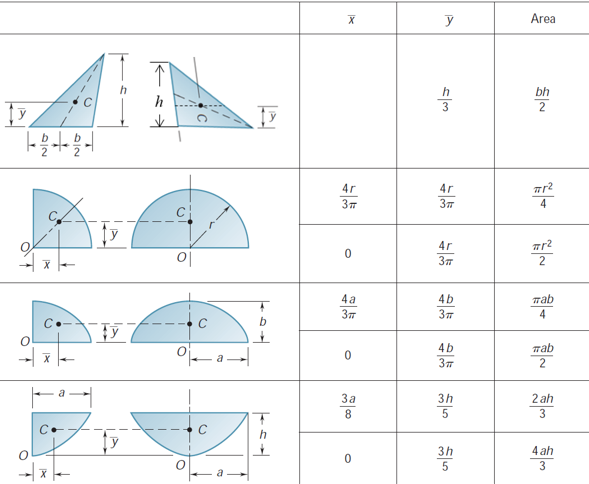
\includegraphics[width=1\linewidth]{screenshot001}
			\label{fig:screenshot001}
			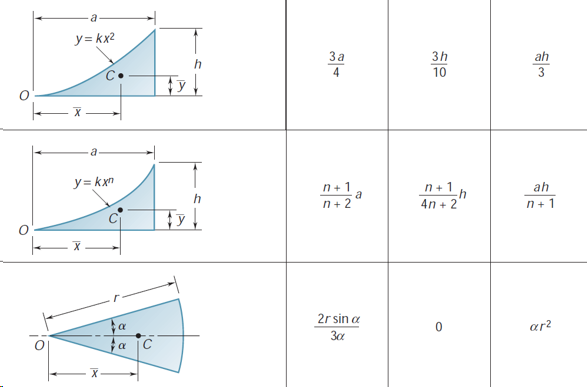
\includegraphics[width=1\linewidth]{screenshot002}
			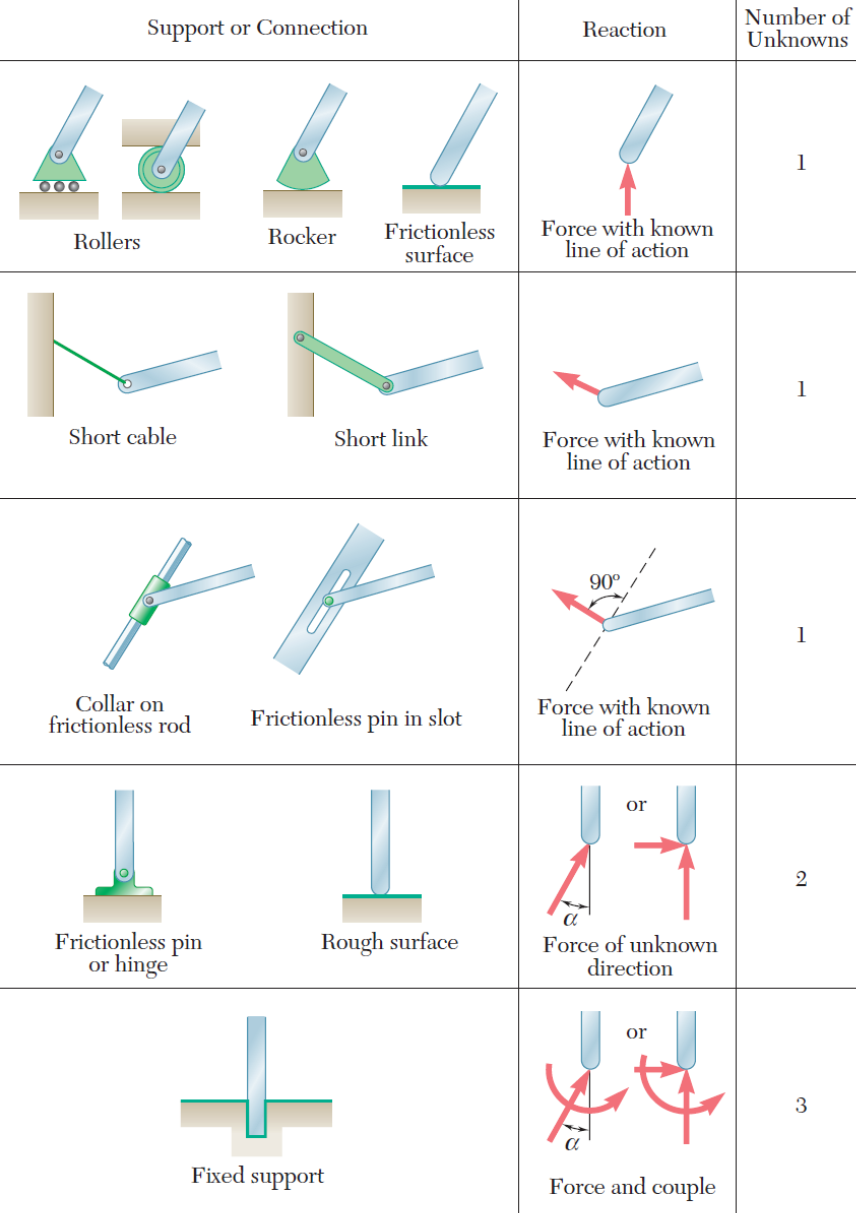
\includegraphics[width=0.7\linewidth,angle=90]{screenshot006}
			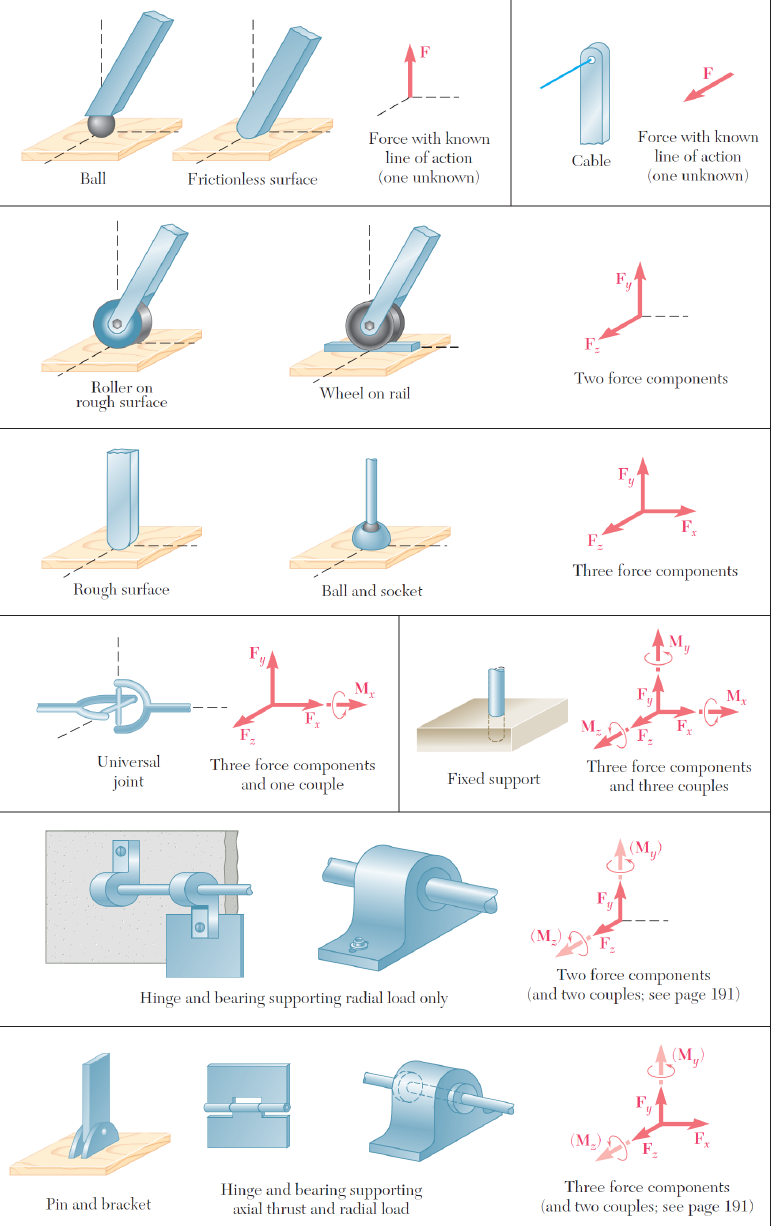
\includegraphics[width=0.7\linewidth,angle=90]{screenshot007}
		\end{figure}
		\begin{figure}[H]
			\centering
			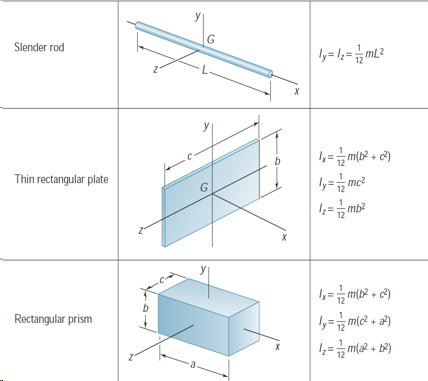
\includegraphics[width=0.9\linewidth]{screenshot003}
			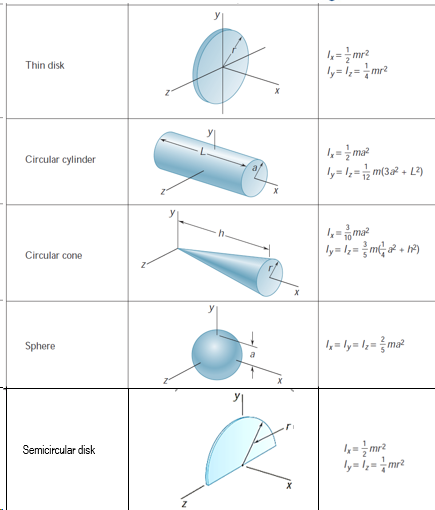
\includegraphics[width=0.9\linewidth]{screenshot004}
			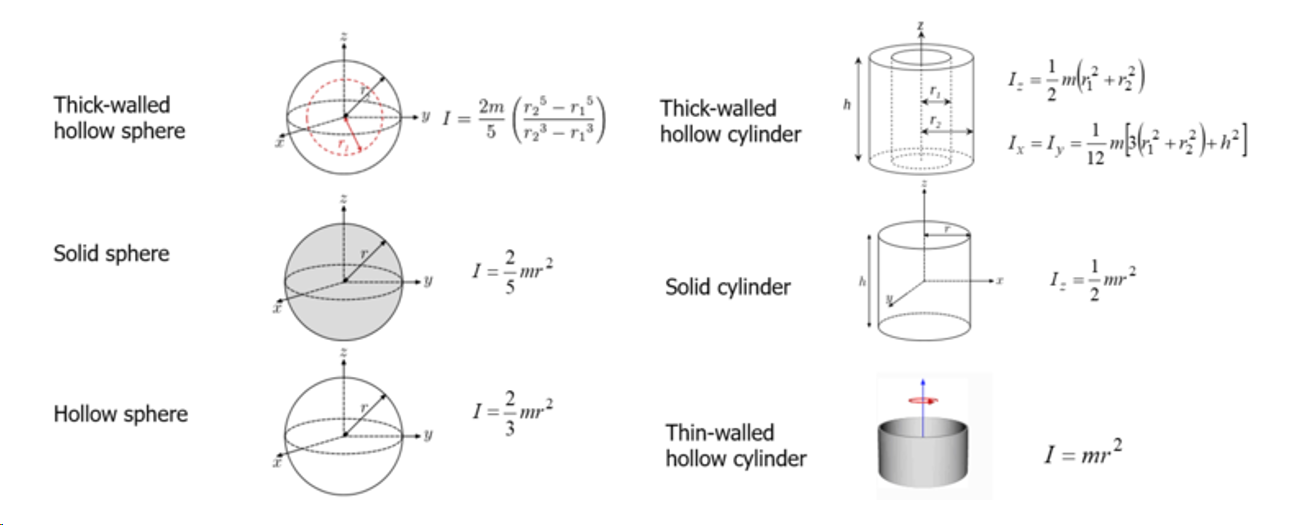
\includegraphics[width=1\linewidth]{screenshot005}
			
			\label{fig:screenshot003}
		\end{figure}
	\end{multicols*}
\end{document}
